\section{Ainul Filiani}
\begin{enumerate}
\item Apa itu fungsi library matplotlip ?

Data yang kita olah tentu tidak bagus apabila ditampilkan begitu saja dengan tabel hitam saja kepada investor atau manajemen. Bila ditampilkan dengan sejumlah grafik berwarna pasti akan terlihat lebih menarik ketika melihatnya. Matplotlib membantu kita untuk memvisualisasikan data dengan lebih indah dan rapi.
Ada plot untuk menampilkan data dengan cara 2D atau 3D. Sehingga kita dapat menampilkan data yang telah kita olah sesuai kebutuhan. Matplotlib pun terintegrasi dengan iPython Notebook atau Jupyter dimana kita dapat membuat sebuah buku interaktif yang dapat diberi penjelasan dan kode yang disisipkan begitupun hasil plottingnya.
Matplotlib adalah library paling banyak atau sering digunakan oleh data science untuk menyajikan datanya ke dalam visual yang lebih baik.

\item jelaskan langkah-langkah membuat sumbu X dan Y di matplotlip?

untuk membuat sumbu x dan y kita bisa menggunakan list untuk mempermudah penyimpanan nilai setiap sumbunya.
contoh pembuatannya: 
\lstinputlisting[firstline=9, lastline=10]{src/6/1174073/teori/1174073.py}

\item jelaskan bagaimana perbedaan fungsi dan cara pakai untuk berbagai jenis (bar, histogram, dll). jenis plot di matplotlip ?  

Untuk perbedaan fungsi plot yang digunakan adalah bentuk bentuk grafik yang akan di tampilkan sesuai dengan perintah yang digunakan pada pemogramannya.
Dan untuk cara pengguna plot tersebut sebagai berikut
\begin{itemize}
    \item line
    Perintah yang digunakan untuk membuat grafik line sebagai berikut.
    \lstinputlisting[firstline=12, lastline=14]{src/6/1174073/teori/1174073.py}
    \item bar
    Dalam Penggunaan plot bar koordinat x nya itu yang awal, dan untuk Y nya adalah yang kedua
    \lstinputlisting[firstline=16, lastline=25]{src/6/1174073/teori/1174073.py}
    \item histogram
    Dalam penggunaan plot histogram titik x nya bisa tidak sama dengan titik Y.
    untuk penggunaannya bisa sebagai berikut.
    \lstinputlisting[firstline=27, lastline=34]{src/6/1174073/teori/1174073.py}
    \item scatter
    Untuk penggunaa plot scatter atau bisa juga d bilang diagram titik.
    Contoh dari penggunaannya bisa dilihat sebagai berikut.
    \lstinputlisting[firstline=36, lastline=49]{src/6/1174073/teori/1174073.py}
    \item Stack plot
    Untuk penggunaan stack plot ini seperti diagram line, tapi ada fill colornya,jadi antar line itu bisa berdekatan.
    Berikut Contoh penggunaannya
    \lstinputlisting[firstline=82, lastline=92]{src/6/1174073/teori/1174073.py}
\end{itemize} 

\item Jelaskan bagaimana cara menggunakan legend dan lebel serta kaitannya dengan fungsi tersebut 

Untuk menggunakan legend dan label bisa di lihat dibawah ini
\lstinputlisting[firstline=20, lastline=22]{src/6/1174073/teori/1174073.py}
penggunaan legend itu untuk mempermudahkita dalam membaca grafik, legend itu sendiri berisi info info dari grafik yang ada seperti nama, kemudian bentuk dan warna.
kemudian untuk label itu sendiri digunakan untuk membedakan nama titik X dan titik Y.

\item Jelaskan apa fungsi dari subplot di matplotlib dan agaimana cara kerja dari fungsi subplot, sertakan ilustraasi dan gambar sendiri dan apa parameternya jika ingin menggambar plot dengan 9 subplot didalamnya ? 

fungsi dari subplot dari matplotlib untuk bisa membuat lebih dari 1 grafik dalam sebuah program.
untuk cara kerjanya sendiri bisa d cek sebagai berikut
\lstinputlisting[firstline=94, lastline=104]{src/6/1174073/teori/1174073.py}
untuk parameternya sendiri saya menggunakan x dan y x sebagai koordinat x dan y sebagai koordinat y.
\begin{figure}[H]	
    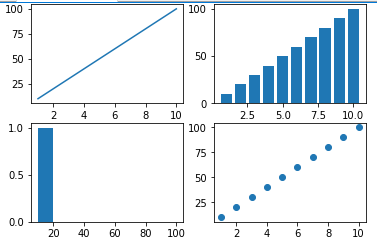
\includegraphics[width=5cm]{figures/6/1174073/teori/satu.png}
    \centering
    \caption{SubPlot}
\end{figure}

\item sebutkan semua pparameter color yang bisa digunakan contoh: m,c,r,k,...

Untuk parameter color yang bisa digunakan terdiri dari 2 type warna.

Tipe Warna RGB

Untuk keterangannya sebagai berikut
\begin{enumerate}
\item R untuk warna Red atau Merah
\item G untuk warna Green atau Hijau
\item B untuk warna Blue atau Biru
\end{enumerate}
Tipe warna CMYK

Untuk keterangannya sebagai berikut
\begin{enumerate}
\item    C untuk warna Cyan atau Biru Muda
\item    M untuk warna Mangenta atau Merah Tua
\item    Y untuk warna Yellow Atau Kuning
 \item   K untuk warna blacK atau Hitam
\end{enumerate}

\item Jelaskan bagaimana cara kerja dari fungsi hist, sertakan ilustrasi dan gambar sendiri?

Untuk fungsi histogram ini kedua titik koordinat boleh tidak sama. Misalnya x nya ada 10 nilai sedangkan Y nya ada 5 nilai, itu tidak akan jadi masalah karena diagram ini digunakan untuk mendata usia dari rentang tertentu atau kebutuhan lainnya.
Ini merupakan contoh dari penggunaan histogram
\lstinputlisting[firstline=27, lastline=34]{src/6/1174073/teori/1174073.py}
dan ini merupakan grafik histogram tersebut.
\begin{figure}[H]	
    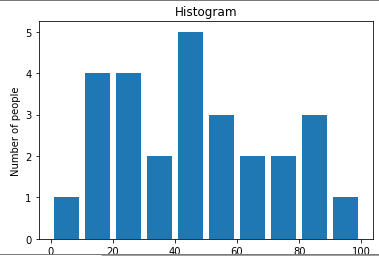
\includegraphics[width=5cm]{figures/6/1174073/teori/histogram.png}
    \centering
    \caption{Diagram Histogram}
\end{figure}

\item jelaskan lebih mendalam tentang parameter dari fungsi pie diantaranya labels, colors,startangle, shadow, explode, autopct.

Berikut penjelasan tentang parameter yang ada dalam pie chart
\begin{itemize}
    \item label
    Label digunakan untuk mempermudah pembaca dalam membaca diagram pie
    \item color
    warna digunakan untuk membedakan antar data
    \item startangle
    Digunakan untuk sudut yang digunakan untuk memulai diagram pie tersebut
    \item shadow
    bayangan digunakan untuk membuat bayangan dari setiap diagram pie yang menonjol
    \item explode
    explode digunakan untuk mengeluarkan suatu data agar data tersebut terlihat menonjol
    \item autopct
    Digunakan sesuai dengan berapa angka dibelakang koma yang kita inginkan
\end{itemize} 
\end{enumerate}
%%%%%%%%%%%%%%%%%%%%%%%%%%%%%%%%%%%%%%%%%%%%%%%%%%%%%%%%%%%%%%%
\section{Sekar Jasminei}
\begin{enumerate}

\item 1. Apa itu fungsi library Matplotlib
Matplotlib adalah sebuah library pada python yang digunakan untuk membuat diagram. Library ini biasanya menghasilkan ploting 2D.\\

Ada plot untuk menampilkan data secara 2D atau 3D. sehingga kamu dapat menampilkan data yang telah kamu olah sesuai kebutuhan. Matplotlib pun terintegrasi dengan ipython notebook atau jupyter dimana kamu dapat membuat sebuah buku interaktif yang dapat diberi penjelasan dan kode yang disisipkan begitupun hasil plottingnya.\\

\item 2. Jelaskan langkah-langkah membuat sumbu X dan Y di matplotlib.
untuk membuat sumbu x dan y kita bisa membuatnya menggunakan list untuk mempermudah penyimpanan nilai setiap sumbunya.\\
\lstinputlisting[firstline=9, lastline=11]{src/6/1174075/teori/1174075.py}

\item 3. Jelaskan bagaimana perbedaan fungsi dan cara pakai untuk berbagai jenis(bar,histogram,scatter.dll) jenis plot di matloptlib
Untuk perbedaan fungsi plot yang digunakan adalah bentuk bentuk grafik yang akan di tampilkan sesuai dengan perintah yang digunakan pada pemogramannya.\\

line itu untuk perintah yang digunakan untuk membuat grafik line sebagai berikut.\\
\lstinputlisting[firstline=12, lastline=15]{src/6/1174075/teori/1174075.py}
Bar itu di dalam Penggunaan plot bar koordinat x nya itu yang awal, dan untuk Y nya adalah yang kedua.\\
\lstinputlisting[firstline=16, lastline=26]{src/6/1174075/teori/1174075.py}
Histrogram itu di dalam penggunaan plot histogram titik x nya bisa tidak sama dengan titik Y. untuk penggunaannya bisa sebagai berikut.\\
\lstinputlisting[firstline=27, lastline=35]{src/6/1174075/teori/1174075.py}
scatter untuk penggunaa plot scatter atau bisa juga d bilang diagram titik.\\
\lstinputlisting[firstline=36, lastline=50]{src/6/1174075/teori/1174075.py}
Stack plot untuk penggunaan stack plot ini seperti diagram line, tapi ada fill colornya,jadi antar line itu bisa berdekatan.\\
\lstinputlisting[firstline=82, lastline=92]{src/6/1174075/teori/1174075.py}

\item 4. Jelaskan bagaimana cara menggunakan legend dan label serta kaitannya dengan fungsi tersebut.
Contoh source code lengkap disertai dengan link "editor" untuk mencoba (try it) dan melihat hasil (preview) kode.\\

Elemen yang akan ditambahkan ke legenda ditentukan secara otomatis, ketika Anda tidak memberikan argumen tambahan.\\

Garis-garis spesifik dapat dikecualikan dari pemilihan elemen legenda otomatis dengan mendefinisikan label dimulai dengan garis bawah.\\

\item 5. Jelaskan apa fungsi dari subplot di matplotlib dan fungsi dari subplot dari matplotlib untuk bisa membuat lebih dari 1 grafik dalam sebuah program.\\

Misalnya, kita dapat membuat sumbu inset di sudut kanan atas sumbu lain dengan mengatur posisi x dan y ke 0,65 yaitu, mulai dari 65 peren dari lebar dan 65 persen  dari ketinggian gambar dan x dan y meluas ke 0,2 yaitu, ukuran sumbu adalah 20 persen  dari lebar dan 20persen dari tinggi gambar.\\

Simple Grids of Subplots itu kebutuhan yang cukup umum sehingga Matplotlib memiliki beberapa rutinitas kenyamanan yang membuatnya mudah dibuat. Level terendah adalah plt.subplot (), yang membuat subplot tunggal di dalam kisi. Seperti yang Anda lihat, perintah ini membutuhkan tiga argumen bilangan bulat — jumlah baris, jumlah kolom, dan indeks plot yang akan dibuat dalam skema ini, yang berjalan dari kiri atas ke kanan bawah.\\

The Whole Grid in One Go itu  membuat grid besar subplot, terutama jika Anda ingin menyembunyikan label sumbu x dan y pada plot bagian dalam. Untuk tujuan ini, plt.subplots () adalah alat yang lebih mudah digunakan.\\
\lstinputlisting[firstline=94, lastline=104]{src/6/1174075/teori/1174075.py}
 
\item 6. Sebutkan semua parameter color yang bisa digunakan(contoh: m,c,r,k,...dkk)
Tipe Warna RGB
    Untuk keterangannya sebagai berikut
    R untuk warna Red atau Merah
    G untuk warna Green atau Hijau
    B untuk warna Blue atau Biru.\\
    
Tipe warna CMYK
    Untuk keterangannya sebagai berikut
    C untuk warna Cyan atau Biru Muda
    M untuk warna Mangenta atau Merah Tua
    Y untuk warna Yellow Atau Kuning
    K untuk warna blacK atau Hitam.\\

\item 7. Jelaskan bagaimana cara kerja dari fungsi hist , sertakan ilustrasi dan gambar sendiri.
Untuk fungsi histogram ini kedua titik koordinat boleh tidak sama. Misalnya x nya ada 10 nilai sedangkan Y nya ada 5 nilai, itu tidak akan jadi masalah karena diagram ini digunakan untuk mendata usia dari rentang tertentu atau kebutuhan lainnya.\\

Ini merupakan contoh dari penggunaan histogram.\\

\item 8. Jelaskan lebih dalam tentang parameter dari fungsi pie diantaranya labels , color , startangle , shadow , explode , autopct.
Jika jumlah x <1, maka nilai x memberikan area fraksional secara langsung dan array tidak akan dinormalisasi.\\

labels : Label digunakan untuk mempermudah pembaca dalam membaca diagram pie.\\

color : warna digunakan untuk membedakan antar data.\\

startangle : Digunakan untuk sudut yang digunakan untuk memulai diagram pie tersebut.\\

shadow :  bayangan digunakan untuk membuat bayangan dari setiap diagram pie yang menonjol.\\

explode : explode digunakan untuk mengeluarkan suatu data agar data tersebut terlihat menonjol.\\

autopct : Digunakan sesuai dengan berapa angka dibelakang koma yang kita inginkan.\\
\end{enumerate}
%%%%%%%%%%%%%%%%%%%%%%%%%%%%%%%%%%%%%%%%%%%%%%%%%%%%%%%%%%%%%%%%%%%%%%%%%%%%%%%%%%%%%%%%%%%%%%%%%%%

\section{Kaka Kamaludin}
\subsection{Soal 1}
Matplotlib merupakan library python yang berfungsi untuk mengasilkan plot yang di paparkan dengan toolkit GUI yang interaktif.

\subsection{Soal 2}
penulisan Sumbu x dan Y, pada plt.plot(xxx, yyy) diwali dengan sumbu x lalu y.
\lstinputlisting[firstline=1, lastline=13]{src/6/1174067/Teori/1174067_teori.py}


\subsection{Soal 3}
\begin{itemize}
	\item Line Plot, berfungsi untuk menamplikan data yang berkelanjutan dalam priode tertentu.
	\lstinputlisting[firstline=15, lastline=18]{src/6/1174067/Teori/1174067_teori.py}
	
	\item Pie Chart, berfungsi untuk menamplikan bagian suatu data terhadap jumlah keseluruhan secara proporsional. 	setiap bagian data dihitung dalam persentase. pie chart berbentuk bulat seperti potongan kue.
	\lstinputlisting[firstline=20, lastline=42]{src/6/1174067/Teori/1174067_teori.py}
	
	\item Bar Chart, berfungsi sebagai perbandingan beberapa kategori data, ditampilkan dalam bentuk batang.
	\lstinputlisting[firstline=43, lastline=53]{src/6/1174067/Teori/1174067_teori.py}
	
	\item Scatter Chart, biasa digunakan untuk pengujian pola hubungan antara dua variable.
	\lstinputlisting[firstline=54, lastline=69]{src/6/1174067/Teori/1174067_teori.py}
	
	\item Histogram Chart, berfungsi untuk perbandingan data dalam bentuk range.
	\lstinputlisting[firstline=70, lastline=79]{src/6/1174067/Teori/1174067_teori.py}
	
	\item Stack Chart,.
	\lstinputlisting[firstline=80, lastline=101]{src/6/1174067/Teori/1174067_teori.py}		
\end{itemize}

\subsection{Soal 4}
Legend dan Label berfungsi untuk mempermudah dalam pembacaan chart tersebut. contohnya:
\lstinputlisting[firstline=102, lastline=119]{src/6/1174067/Teori/1174067_teori.py}

\subsection{Soal 5}
sublpot berfungsi untuk membuat plot lebih dari 1, contoh:
\lstinputlisting[firstline=120, lastline=148]{src/6/1174067/Teori/1174067_teori.py}

\subsection{Soal 6}
parameter color bisa dibuat dengan menggunakan float value(0.1, 0.2, 0.5, 0.3), hex ('\# 0F0F0F' atau '\#0F0F0F0F'), xkcd color ('xkcd:sky blue'), Tableau Colors ('tab:gray')
\begin{itemize}
    \item Tipe Warna RGB

    R untuk warna Red atau Merah,
    G untuk warna Green atau Hijau,
    B untuk warna Blue atau Biru,
    \item Tipe warna CMYK

    C untuk warna Cyan atau Biru Muda,
    M untuk warna Mangenta atau Merah Tua,
    Y untuk warna Yellow Atau Kuning,
    K untuk warna black atau Hitam
\end{itemize}
\lstinputlisting[firstline=149, lastline=169]{src/6/1174067/Teori/1174067_teori.py}

\subsection{Soal 7}
Untuk fungsi histogram ini kedua titik koordinat boleh tidak sama. Misalnya x nya ada 10 nilai sedangkan Y nya ada 5 nilai, itu tidak akan jadi masalah karena diagram ini digunakan untuk mendata usia dari rentang tertentu atau kebutuhan lainnya.
	\lstinputlisting[firstline=170, lastline=177]{src/6/1174067/Teori/1174067_teori.py}

\subsection{Soal 8}
\begin{itemize}
    \item label
    Label digunakan untuk mempermudah pembaca dalam membaca diagram pie
    \item color
    warna digunakan untuk membedakan antar data
    \item startangle
    Digunakan untuk sudut yang digunakan untuk memulai diagram pie tersebut
    \item shadow
    bayangan digunakan untuk membuat bayangan dari setiap diagram pie yang menonjol
    \item explode
    explode digunakan untuk mengeluarkan suatu data agar data tersebut terlihat menonjol
    \item autopct
    Digunakan sesuai dengan berapa angka dibelakang koma yang kita inginkan
\end{itemize}

%%%%%%%%%%%%%%%%%%%%%%%%%%%%%%%%%%%%%%%%%%%%%%%%%%%%%%%%%%%%%%%%%%%%%%%%%%%%%%%%%%%%%%%%%%%%%%%%%%%